\documentclass[12pt]{article}
\usepackage{amsmath}
\usepackage{epsfig,psfrag}
\usepackage{natbib}
\usepackage{graphicx}
\usepackage[shortlabels]{enumitem}
\setlength{\textwidth}{6.5in}
\setlength{\textheight}{8.9in}
\setlength{\voffset}{-1in}
\setlength{\oddsidemargin}{0in}
\setlength{\evensidemargin}{0in}

%biblography of JFM Style
\bibliographystyle{jfm}

%Some mathematical Definitions
\def\o{\over}
\def\p{\partial}
\def\be{\begin{eqnarray}}
\def\ee{\end{eqnarray}}
\def\bes{\begin{subeqnarray}}
\def\ees{\end{subeqnarray}}

\def\f{\frac}
\def\lp{\left(}
\def\rp{\right)}
\def\lb{\left[}
\def\rb{\right]}
\def\lcb{\left\{}
\def\rcb{\right\}}
\def\n{\nabla}
\def\lap{\nabla^2}
\def\z{\zeta}
\def\ep{\epsilon}
\def\l{\lambda}
\def\befi{\begin{figure}}
\def\eefi{\end{figure}}
\def\a{\alpha}
\def\no{\noindent}
\def\h{\hat{}}
\def\bce{\begin{center}}
\def\ece{\end{center}}



\def\d{\text{d}}
\def\vep{\varepsilon}
\def\ep{\epsilon}
\def\la{\langle}
\def\ra{\rangle}
\def\th{\theta}


\title{Percolation}
\author{Ahmad}
%-------------------------------------------------------------------
\begin{document}          
\maketitle


\section{Permeability modification Model}
%
The polymers passing through pores are dragged by the flow. There are
two forces competing when a polymer adheres to the surface of a pore
(1) The drag force on the particle coming from flow, and (2)
ionic/VanderWaals or whatever force that tries to adhere the particles
to the surface. A particle attaches to the surface if the drag force
exerted by the fluid flow around it is smaller than the
VanderWaals/ionic force.

For simplicity, I assume that the force is ionic with a force distance
profile of $F= K/X^2$, where $K$ is a constant and $X$ is the
distance. I assume that polymers have an effective radius of $d_{p}$
and fluid viscosity is $\mu$ and the flow rate is $Q$. This model
states that the particle attaches to the surface when
%%
\begin{align}
    F_{\text{drag}} &\leq F_{\text{ionic}}\\
    6\pi \mu d_{p} \frac{2Q}{\pi R^2} \lp 1- \frac{r^2}{R^2} \rp & \leq \frac{K}{(R-r)^2} \\
    1 - \frac{r^2}{R^2} & \leq \lp \frac{K }{12 \mu  d_{p} Q} \rp \frac{1}{\lp 1 - r/R \rp^2} \\
    1 & \leq \frac{r^2}{R^2} + \alpha \frac{1}{\lp 1-r/R\rp ^2}
\end{align}
%
where $\alpha = K/\lp 12\mu d_pQ \rp$ is a factor that compares the ionic force and viscous
force. Note that it depends on the flux rate. If we define
$x = 1- r/R$ we obtain
%
\begin{align}
    1 &\leq (1-x)^{2} + \frac{\alpha}{x^2} \\
    x^2- x^2(1-x)^{2} &\leq \alpha \\
    x^2 (1- (1-x)^2) & \leq \alpha \\
    x^3(2-x) & \leq \alpha \\
    \text{if } x\ll1 \to x & \leq \lp \frac{\alpha}{2}\rp^{1/3}
\end{align}
%
%
\begin{figure}[h]
  \centering
  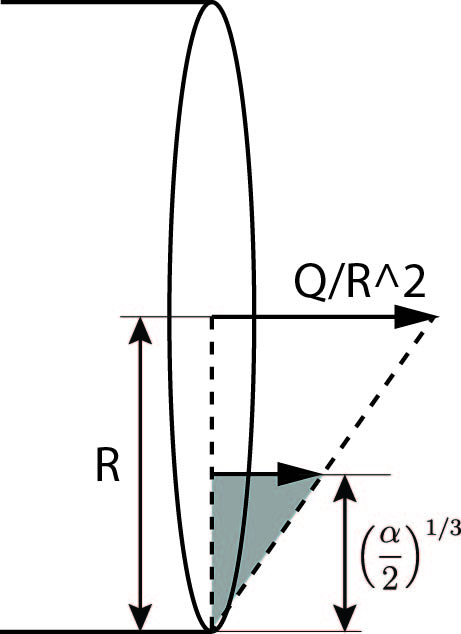
\includegraphics[width=4cm]{./Figs/model2.jpg}
  \caption{Flow in the pipe}
\end{figure}
%
As a result the distance is proportional to $\alpha^{1/3}$. Note that
$\alpha$ depends on $1/Q$.  Now, lets
find the flux passing through this adsorbtion layer (any polymer in
this layer would attach to the surface)
%
%
\begin{align}
  \text{volume}/\text{time} &= \frac{1}{2} R \alpha ^{1/3} \cdot \frac{Q}{R^{3}} R\a^{1/3} \cdot 2\pi R = \pi Q \a^{2/3}  = \pi \lp \frac{K  }{12 \mu  d_{p}} \rp^{2/3} Q^{1/3} \\
  \text{volume}/\text{time} & \propto {Q^{1/3}} 
\end{align}
%
Now, if we assume that the number of polymers passing through the area
cause clogging of the pipe and change the total area of the pipe, then
we find that

%
\begin{align}
  d (\pi R^2) \propto Q^{1/3} \quad \to \quad R dR \propto Q^{1/3}
\end{align}
%
We also know that $k = \pi R^4/8l^2$, as a result
%
\begin{align}
  dk \propto R^{3} dR \\
  dk \propto R^2 Q^{1/3} \\
  dk \propto Q^{1/3}
\end{align}

\subsection*{Experimental Results}
%
In Shima's paper, we report a figure that shows the evolution of
permeability $k$ per volume of polymer $V_{pol}$ that passes through
the porous media. Basically we are plotting $\Delta k$ versus $Q$
passing through the porous media. The figure and best polynomial fit
is shown blow
%
%
\begin{figure}[h]
  \centering
  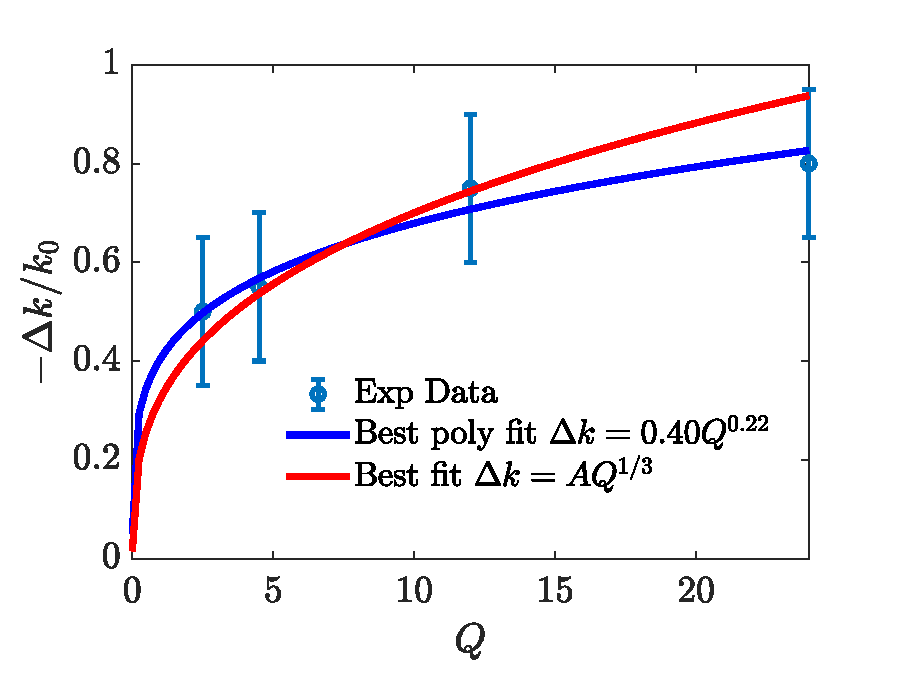
\includegraphics[width=0.55\textwidth]{./Figs/k-evolution.eps}
  \caption{$k$ versus volume of fluid}
\end{figure}





\newpage
\newpage
\newpage






\section{Universality argument}

If the pdf of $q$ follows an exponential tail, we have
%
\begin{align}
  f(q) \propto e^{-q/\lambda}
\end{align}
%
Doing the normalization, we find that
%
\begin{align}
  f(q) = \frac{1}{\lambda} e^{-q/\lambda} \text{such that} \int f(q) dq = 1
\end{align}
%
Setting the average $\langle Q \rangle = Q_0$, we obtain
%
\begin{align}
  \int q f(q) dq = \lambda = Q_{0}
\end{align}
%
We then obtain
%
\begin{align}
  f(q) = \frac{1}{Q_{0}} e^{-q/Q_0}
\end{align}
%
This means that as long as $Q_0$ is fixed, then the probability
distribution is fixed. However, the observation is that as the
clogging happens, the $f(q)$ broadens! 

\section{Random Resistor Networks}
%
Consider the following random network
%
%
\begin{figure}[h]
  \centering
  \includegraphics[width=12cm]{./Figs/grid.eps}
  \caption{A random grid of pipes} \label{fig-grid}
\end{figure}
%
The diameter of each pipe is randomly chosen from a distribution
distribution. The Darcy law in each pipe reads as
%
\begin{align}
  \frac{\Delta P}{L}  = \frac{128}{\pi} \frac{\mu Q}{d^4} 
\end{align}
%
where $\Delta P$ is the pressure difference on both sides of the pipe,
$L$ is the length of the pipe, $\mu$ is viscosity, and $d$ is the
diameter of the pipe.
% 



\section{Analysis}
%
Consider the following random network of pipes
%
\begin{figure}[h]
  \centering
  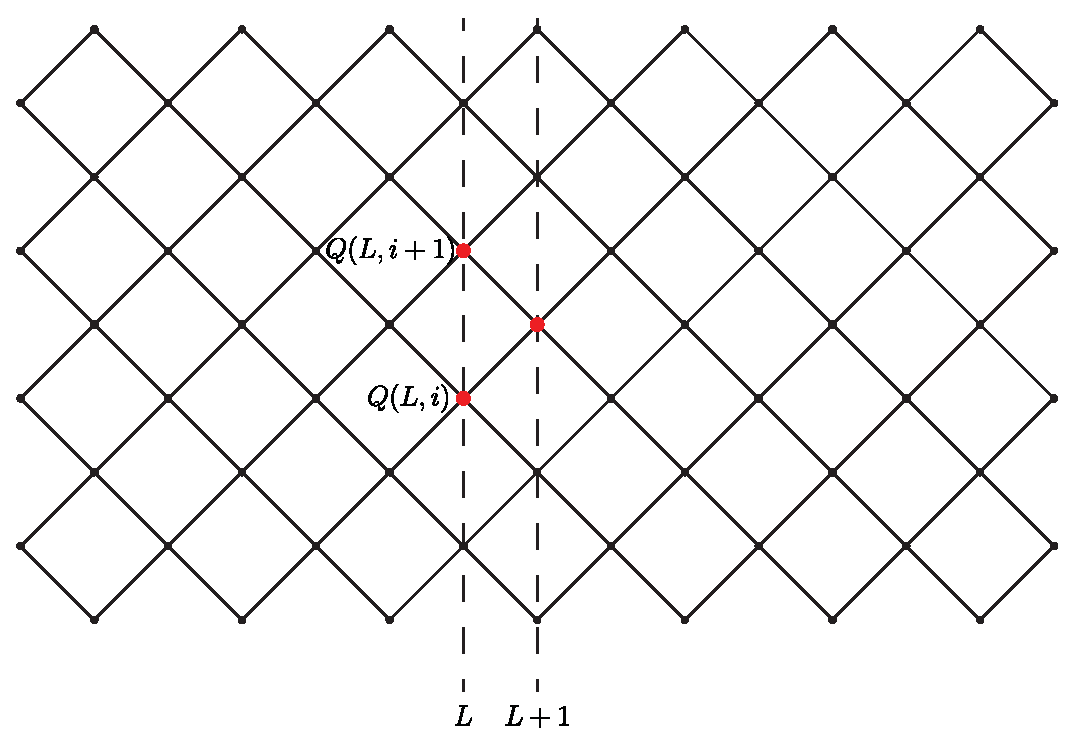
\includegraphics[width=12cm]{./Figs/grid2.eps}
  \caption{A random grid of pipes} \label{fig-grid}
\end{figure}
%
At each level, at each node, the flow from previous layers into that
node is considered as $Q(L,i)$.  This flow goes to the next layer
through the pipes that it is connected to. Some portion of it flows
through each pipe as
%
\begin{align}
  Q(L+1,j) = \sum_i w_{ij} Q(L,i) = w_{i,i+1} Q(L,i+1) + w_{i,i} Q(L,i) 
\end{align}
%
such that $\sum_{j} w_{ij} = 1$. Assuming that these $w_{ij}$ are
coming from a distribution $\eta(w)$, we know that
%
\begin{align}
 \boxed{ \int \eta(w) dw = 1 }
\end{align}
%
and from $\sum_jw_{ij} = 1$, we can conclude that
%
\begin{align}
  \sum_j w_{ij}=1 \to N {E}[w_{ij}] = 1 \to E[w_{ij}] = 1/N \to \boxed{\int w\eta(w) dw = 1/N}
\end{align}
%

Now we use the technique of mean field analysis for a general
distribution of $\eta(w)$ to find the distribution of $Q$ at the
layers. The values of $Q(D,i)$ are not independent for neighboring
sites; however, the mean field approximation ignores these
correlations.
%
\begin{align}
  P_L (Q) = \prod_{j=1}^N \left\{ \int_0^1 d w_j \eta(w_j) \int_0^{\infty} dQ_j P_{L-1}(Q_j)\right\} \times \delta \lp \sum_j w_j Q_{j} - Q \rp
\end{align}
%
The constraint that $Q$'s eminating downward should add up to one is
in the definition of $\eta(w)$. The only approximation in the above
equation is that we neglect the possible correlation between the
values of $Q$ among anscestors. If we take the laplace transform of
the above equation, we obtain
%
\begin{align}
  \tilde P(s) & \equiv \int_0^{\infty} P(Q) e^{-Qs} dQ\\
  \xrightarrow{\int_0^{\infty} (\cdot) e^{-Qs} dQ}  P (Q) & = \prod_{j=1}^N \left\{ \int_0^1 d w_j \eta(w_j) \int_0^{\infty} dQ_j P(Q_j)\right\} \times \delta \lp \sum_j w_j Q_{j} - Q \rp \\
  \tilde P(s) & = \int_0^{\infty} \prod_{j=1}^N \left\{ \int_0^1 d w_j \eta(w_j) \int_0^{\infty} dQ_j P(Q_j)\right\} \times \delta \lp \sum_j w_j Q_{j} - Q \rp e^{-Qs}dQ \\
              & = \prod_{j=1}^N \left\{ \int_0^1 d w_j \eta(w_j) \int_0^{\infty} dQ_j e^{-\sum w_{j}Q_{j}} P(Q_j)\right\}   \\
              & = \prod_{j=1}^N \left\{ \int_0^1 d w_j \eta(w_j) \tilde P(s w_j) \right\} \\
  & = \lp  \int_0^1 d w \eta(w) \tilde P(s w)  \rp^{N}
\end{align}
%
Or to summarize
%
\begin{align}
  \tilde P(s) = \lp  \int_0^1 d w \eta(w) \tilde P(s w)  \rp^{N} \label{eq:main-laplace}
\end{align}
%
Note that in the above calculation $N=2$. If we set $\eta(w) =
\delta(w-1/2)$, then the flow at each node has probality of $1/2$ to
move up or down. As a result the flow at a given depth $L$ will be
homogeneous as $P_L(Q) = \delta (Q-\bar{Q})$ where $\bar{Q}$ is the
average of input fluid flow.

\subsection*{$P(Q)$ decays faster than $Q^{-n}$ for any $n$}
We first show that $P(Q)$ decays faster than any power of $Q$ for any
weight distributions. We expand the Laplace transform as
%
\begin{align}
  \tilde P(s) = 1 + \sum_j \tilde P_{j} s^{j}
\end{align}
%
Inserting this expansion into Eq. \eqref{eq:main-laplace}, we obtain
%
\begin{align}
  1 + \sum_j \tilde P_{j} s^{j}  & = \lp  \int_0^1 d w \eta(w) \lb 1 + \sum_j \tilde P_{j} (sw)^{j}\rb    \rp^{N} \\
 & = \lp  1 + \sum_j \tilde P_j \langle w^{j}\rangle  s^{j}   \rp^{N}
\end{align}
%
where $\langle w^j \rangle = \int_0^1 \eta(w) w^j dw$ is the $j$-th
moment of the weights $w$. In the above equation we can observe that
%
\begin{align}
  P_j \lp N \langle w^j\rangle -1 \rp = G(P_{j-1}, P_{j-1}, \cdots, P_1)
\end{align}
%
In the above equation $P_j$ can only diverge only if $N\langle w^j
\rangle -1$ is zero. If $w$ can only be zero and one, then $\langle
w^j\rangle =\langle w \rangle = 1/N$ and the coefficient can become
zero! Other than this special distribution where $0 \leq w \leq 1$,
then
%
\begin{align}
  & w\in [0,1] \rightarrow w>w^2>w^3> \cdots \\
  & \forall k>1 \rightarrow \langle w^k \rangle < \langle w \rangle = \frac{1}{N} 
\end{align}
%
which means that $N\langle w^j \rangle -1$ is not zero and as a result
$P_j$ is finite. $P_j$ on the other hand is the $j$-th moment or
$\langle Q^j\rangle$ and it is finite. If $P\approx Q^{-n}$, then the
$n$-th moment will not be finite i.e. $\langle Q^{n+1}\rangle =
P_{n+1}$ is not finite. We can then conclude that $P(Q)$ should go to
zero faster than any $Q^{-n}$ as $Q\to \infty$! In other words $d \log
P(Q) / d \log Q \to -\infty$ as $Q\to \infty$.  

\subsection*{Exponential Decay}
%
Since our calculation is for $N=2$, the main equation becomes
%
\begin{align}
  \tilde P(s) = \lp  \int_0^1 d w \eta(w) \tilde P(s w)  \rp^{2} 
\end{align}
%
In order to have an approximation for $\eta(w)$ we do the following:

At each node there are two nodes where the flux is distributed by
$w_1$ and $w_2$. Lets assume that $w_1$ is uniformly distributed
between $0$ and $1$. As a result $w_2 = 1-w_1$ (since conservation of
mass $w_1 + w_2 = 1$). Now $\eta(w)$ can be found as
%
\begin{align}
  & \eta(w) = M \int_0^1 dw_1 \delta(1-w_1-w) =  M, \\
  \text{since }& \int_0^1 \eta(w) dw = 1 \to M =1 \\
  & \eta (w) = 1
\end{align}
%
Just for completeness, if there are three connections ($N=3$), then we
have
%
\begin{align}
  \eta(w) & = M \int_0^1 dw_1 \int_0^1 dw_2 \delta(1-w_1-w_2 - w)\\
          & = M(1-w)  \to \int_0^1\eta(w) dw = 1 \to M = \frac{1}{2} \\
  & \eta(w) = \frac{1}{2} (1-w)
\end{align}
%
As a result the main equation simplifies to
%
\begin{align}
  \tilde P(s) = \lp  \int_0^1 d w  \tilde P(s w)  \rp^{2} 
\end{align}
%
In order to solve the above equation, we assume $\tilde V (s) =
\sqrt{\tilde{P}(s)}$.
%
\begin{align}
  \tilde{V}(s) & = \int_0^1 dw \tilde V (sw) = \int_0^s \frac{du}{s}  \tilde{V}^{2}(u) \\
  s\tilde{V}(s) & = \int_0^s du  \tilde{V}^2(u) \\
\end{align}
%
Taking the defferentiation with respect to $s$ yields
%
\begin{align}
  \tilde{V}(s) + s \frac{d \tilde{V}(s)}{d s} = \tilde{V}^2(s) \\
  \frac{d \tilde{V}}{\tilde{V}^2-\tilde{V}} = \frac{ds}{s}  \\
  \log\lp \frac{1-\tilde{V}}{\tilde{V}} \rp  = \log(s)\\
  \tilde{V}(s) = \frac{1}{1+Cs} 
\end{align}
%
We set the mean to $1$ i.e.,
%
\begin{align}
  \int_0^{\infty} Q P(Q) dQ = 1 \to \frac{d\tilde{P}}{ds}|_{s=0}  = -1\\
  \frac{d \tilde{V}}{ds}  = \frac{1}{2 \sqrt{\tilde{P}(s)}} \frac{d \tilde{P}(s)}{d s}   \to \frac{d\tilde{V}(s)}{ds}|_{s=0} =\frac{-1}{2} \\
  \frac{d\tilde{V}(s)}{ds} = \frac{-C}{(1+Cs)^{2}}|_{s=0} = -C = \frac{-1}{2}  \to C=\frac{1}{2} 
\end{align}
%
As a result, we have
%
\begin{align}
  \tilde{P}(s) = \lp\frac{1}{1+s/2} \rp^2 \\
  P(Q) = 4Q e^{-2Q}
\end{align}



\section{Continuous Model}
%
\section{Analysis}
%
Consider the following random network of pipes
%
In the previous descrete model we found that
%
\begin{align}
  Q(i,j+1) = w_{i-1,j} Q(i-1,j) + w_{i+1,j} Q(i+1,j) 
\end{align}
%
with the constraint that
%
\begin{align}
  w_{i-1,j} + w_{i+1,j} = 1
\end{align}
%
Lets now assume that
%
\begin{align}
  w_{i\pm 1,j}= \frac{1}{2}( 1 \pm v_{i\pm 1,j})
\end{align}
%
with th abive assumption, we find that
%
\begin{align}
  Q(i,j+1) & = \frac{1}{2} \left( 1 - v_{i- 1,j}\right) Q(i-1,j) + \frac{1}{2} \left( 1 + v_{i+ 1,j}\right) Q(i+1,j)  \\
  Q + L_y \frac{\p Q}{\p y } + L^2_y \frac{\p^{2}Q}{\p y^2}  & = \frac{1}{2} (1-v + L_x \frac{\p v}{\p x}  ) \left( Q - L_x \frac{\p Q}{\p x} +   \frac{1}{2} L_x^2 \frac{\p Q^2}{\p x^2}\right) \nonumber\\
 & \qquad   +\frac{1}{2}  (1+v + L_x \frac{\p v}{\p x} )\left( Q + L_x \frac{\p Q}{\p x} + \frac{1}{2}L_x^2 \frac{\p^2 Q}{\p x^2} \right)  \\
  L_y \frac{\p Q}{\p y } & = L_x v \frac{\p Q}{\p x} + L_x \frac{\p v}{\p x} Q + \frac{L^2_x}{2} \frac{\p^{2}Q}{\p x^2}  \\
  \frac{\p Q}{\p y}    & = \frac{L_{x}}{L_{y}} \frac{\p }{\p x} \left( v Q \right)  + \frac{L^2_x}{2L_y} \frac{\p^{2}Q}{\p x^2}  
\end{align}
%
Assuming that $L_x = L_y $(?), we find that
%
\begin{align}
  \frac{\p Q}{\p y}  = \frac{\p}{\p x} \left( v Q\right) + D \frac{\p^{2} Q}{\p x^2}  
\end{align}



\section{Polymer Adsorption Rate}
%
These polymers (particles) in the tube are dragged by the flow. There are two forces competing when a polymer adheres to the surface (1) The drag force on the particle coming from flow, and (2) ionic/VanderWaals or whatever force that tries to adhere the particles to the surface. A particle attaches to the surface if the drag force exerted by the fluid flow around it is smaller than the VanderWaals/ionic force. 


This means that for a particle to adhere to the surface needs to be at a distance from the surface such that the drag force is smaller than the Van-der-Waals force (say $F_0$). If this happens then the polymer with some probability can adhere to the surface and the flow will not drag it away. This means that particles below this critical velocity.


\begin{align}
    v_\text{cr} = \frac{F_0}{6\pi \mu d}
\end{align}
%
Now, we know that the velocity profile is as 
%
\begin{align}
 v(r) = \frac{2Q}{\pi R^2} \lp 1 - \frac{r^2}{R^2}\rp   \\
 v_\text{cr} = \frac{2Q}{\pi R^2} \lp 1 - \frac{r_\text{cr}^2}{R^2}\rp   \\
 \frac{r_\text{cr}^2}{R^2} = 1 - \frac{v_\text{cr} \pi R^2}{2Q}
\end{align}
%
We are interested in the rate of volume of fluid passing between $r_\text{cr}$ and the boundary of the wall. This becomes
%
\begin{align}
    \text{volume}/\text{time} & = \int_{\text{cr}}^R \frac{2Q}{\pi R^2} \lp 1 - \frac{r^2}{R^2}\rp 2\pi r dr \\
    & = \lp \int_0^R - \int_0^{r_\text{cr}}\rp \frac{2Q}{\pi R^2} \lp 1 - \frac{r^2}{R^2}\rp 2\pi r dr \\
    & = Q - {2Q} \frac{r_\text{cr}^2}{R^2} \lp 1 - \frac{r_\text{cr}^2}{2R^2} \rp \\
    & = Q - {Q} \lp 1 - \frac{v_\text{cr} \pi R^2}{2Q} \rp  \lp 1 +  \frac{v_\text{cr} \pi R^2}{2Q}  \rp \\
    & = Q - {Q} \lp 1 - \frac{v^2_\text{cr} \pi^2 R^4}{4Q^2} \rp \\
    & = Q \lp 1-1+\frac{v^2_\text{cr} \pi^2 R^4}{4Q^2} \rp \\
    & = \frac{v^2_\text{cr} \pi^2 R^4}{4Q}
\end{align}
%


Another easy way to reach to the above calculation is the following 
%
\begin{figure}[h]
  \centering
  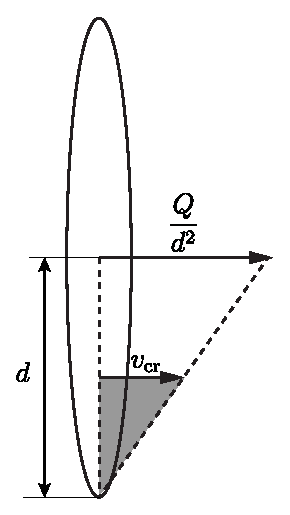
\includegraphics[width=4cm]{./Figs/model1.eps}
  \caption{Flow in the pipe}
\end{figure}
%
The shaded area around the tube can be calculated as 
%
\begin{align}
    \text{volume}/\text{time} = \frac{1}{2} v_\text{cr} \cdot \lp \frac{v_\text{cr}}{q/d^2} d \rp 2 \pi d = \frac{\pi v_\text{cr}^2 d^4}{q}
\end{align}
%
which is upto a factor close to what we obtained earlier. 

\subsection{Modifying the model}
%
For simplicity, let's assume that the force is ionic as $F= K/x^2$. Our model says that
%
\begin{align}
    6\pi \mu d \frac{2Q}{\pi R^2} \lp 1- \frac{r^2}{R^2} \rp & \leq \frac{K}{(R-r)^2} \\
    1 - \frac{r^2}{R^2} & \leq \lp \frac{K \pi }{12 \mu \pi d Q} \rp \frac{1}{\lp 1 - r/R \rp^2} \\
    1 & \leq \frac{r^2}{R^2} + \alpha \frac{1}{\lp 1-r/R\rp ^2}
\end{align}
%
where $\alpha$ is a factor that compares the ionic force and viscous force and it depends on the flux rate. If we define $x = 1- r/R$ we obtain
%
\begin{align}
    1 \leq (1-x)^2 + \frac{\alpha}{x^2} \\
    x^2- x^2(1-x)^2 \leq \alpha \\
    x^2 (1- (1-x)^2) \leq \alpha \\
    x^3(2-x) \leq \alpha \\
    \text{if} x\ll1 \to x\leq \lp \frac{\alpha}{2}\rp^{1/3}
\end{align}
%
As a result the distance is proportional to $\alpha^{1/3}$. 
%
\begin{figure}[h]
  \centering
  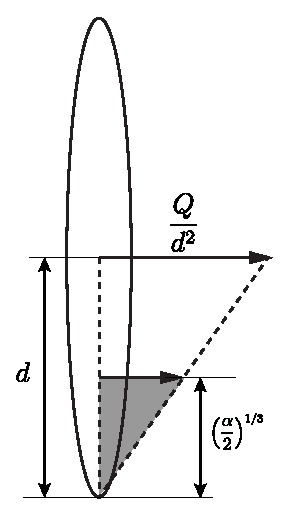
\includegraphics[width=4cm]{./Figs/model2.eps}
  \caption{Flow in the pipe}
\end{figure}
%
Therefore, we obtain
%
\begin{align}
    \text{volume}/\text{time} = \frac{1}{2} \lp \frac{\alpha}{2}\rp^{1/3} \cdot  \frac{Q}{d^3}\lp \frac{\alpha}{2}\rp^{1/3} \cdot 2 \pi d = \frac{\pi}{2^{2/3}} \frac{Q \alpha^{2/3}}{d^2}
\end{align}
%
Note that in here $\alpha$ scales with $1/Q$. 







\section{Derivation of Kozeny-Carman Equation}
%
Assuming a proous material we have
%
\begin{align}
    Q = -k \frac{A}{\mu} \frac{\Delta P}{L}
\end{align}
%
where $Q$ is the flow rate, $\Delta P$ is the pressure difference, $A$ is the cross-sectional area, $\mu$ is the fluid viscosity, and $L$ is the sample length and $k$ is called permeability.


The Kozney-Carman (KC) assumes that a porous media can be represented by a solid block permeated by parallel cylindrical tubes whose axes may be at an angle to the pressure gradient, so that the length of an individual pipe is larger than that of the block. To relate permeability $k$ to porosity in such idealized porous media we need to relate $Q$ to $\Delta P$. Each cylindrical pipe is circular with radius $r$. Poisulle flow for a pipe says 
%
\begin{align}
    Q = - \frac{\pi r^4}{8\mu} \frac{\Delta P}{l}
\end{align}
%
where $r$ is the radius of the pipe and $l$ is the length of the pipe. The porosoity $\phi$ and specific surface area $S$ can be related as 
%
\begin{align}
    \phi = \frac{\pi r^2 l}{A L}  = \frac{\pi r^2}{A } \tau
\end{align}
%
where $\tau$ is known as tortuosity (ratio of total flow path length to length of the sample). 
%
The surface area is then
%
\begin{align}
    S = \frac{2\pi r l}{A L} = \frac{2 \pi r^2 \tau}{A} \frac{1}{r} = \frac{2\phi}{r}
\end{align}
%
Using Poisulle flow in a tube we have
%
\begin{align}
    Q = - \frac{\pi r^4}{8\mu} \frac{\Delta P}{l} = - \frac{\pi r^4}{8A}\frac{L}{l} \frac{A}{\mu} \frac{\Delta P}{L} 
\end{align}
%
As a result the permeability becomes 
%
\begin{align}
    k & = \frac{\pi r^4}{8A} \frac{L}{l} = \frac{\pi r^4}{8A\tau} = \frac{1}{8} \frac{\pi r^2\tau}{A} \frac{1}{\tau^2}r^2 \\
    & = \frac{1}{8} \phi \frac{1}{\tau^2} \lp \frac{2\phi}{S}\rp^2 = \frac{\phi^3}{2S^2 \tau^2}
\end{align}
%
where remember that $S$ is the ratio of the total pore surface to the total volume of the porous sample, and $\tau$ is turtosity $l/L$.  



Now assume $n$ spherical grains with radius $r$, the total volume is $n 4\pi R^3/3$ and the total surface area is $n 4 \pi R^2$. These grains occupy $1-\phi$ of the total volume. As a result we have
%
\begin{align}
    S = \frac{n 4\pi R^2}{4/3 \cdot n \cdot \pi R^3/(1-\phi) } = \frac{3(1-\phi)}{R}
\end{align}
%
putting all back into the equation, we obtain
%
\begin{align}
    k = \frac{\phi^3}{2S^2 \tau^2} = \frac{\phi^3 R ^2}{2\cdot 9 (1-\phi)^2\tau^2} = \frac{R^2}{18 \tau^2} \frac{\phi^3}{(1-\phi)^2}
\end{align}

As we can see in the simulations, the radius of the tubes does not change that much. If you make this equivalency for the tubes, we find that
%
\begin{align}
    S = S \to \frac{2\phi}{r} = \frac{3(1-\phi)}{R}\\
    \phi = 0.48,~~ R = 75\mu m \\
    r = 44\mu m
\end{align}
%
Looking at the voids, we see that the average pore radius in the experiment is only $13\mu m$. How that can be? How can a tube with 3 times the radius represent an average pore size of $13\mu m $. I argue that the void volume should be equal in these two cases.



\section{My Model}
%
\begin{align}
    Q_\text{tube} = - \frac{\pi r^4}{8\mu} \frac{\Delta P_\text{tube}}{l_\text{tube}}
\end{align}
%
Fore each tube. In total we know that
%
\begin{align}
    Q_\text{tot} = n \frac{\pi r^4}{8\mu} \frac{\Delta P_\text{tube}}{l_\text{tube}}
\end{align}
%
where $n$ is the density of the tubes. This density should be proportional to the area divided by the distance between these tubes. 
%
\begin{align}
    Q = \frac{1}{l^2} \frac{\pi r^4}{8} \frac{A}{\mu}\frac{\Delta P}{L}
\end{align}
%
As a result the permeability is 
%
\begin{align}
    k = \frac{\pi r^4}{8l^2}
\end{align}
%
The question now is how to relate this $r$ and $l$ to porosity and radius of packing objects. 

\begin{align}
    \phi = \frac{\frac{A}{l^2} \pi r^2 L}{A L} = \frac{\pi r^2}{l^2}
\end{align}
%
As a result
%
\begin{align}
    k = \frac{l^2}{\pi} \phi^2
\end{align}



\section{Two pipe model}
%
In order to simplify the calculations, we run the two pipe
model. Assume the followig pipe structure
%
\begin{figure}[h]
 \centerline{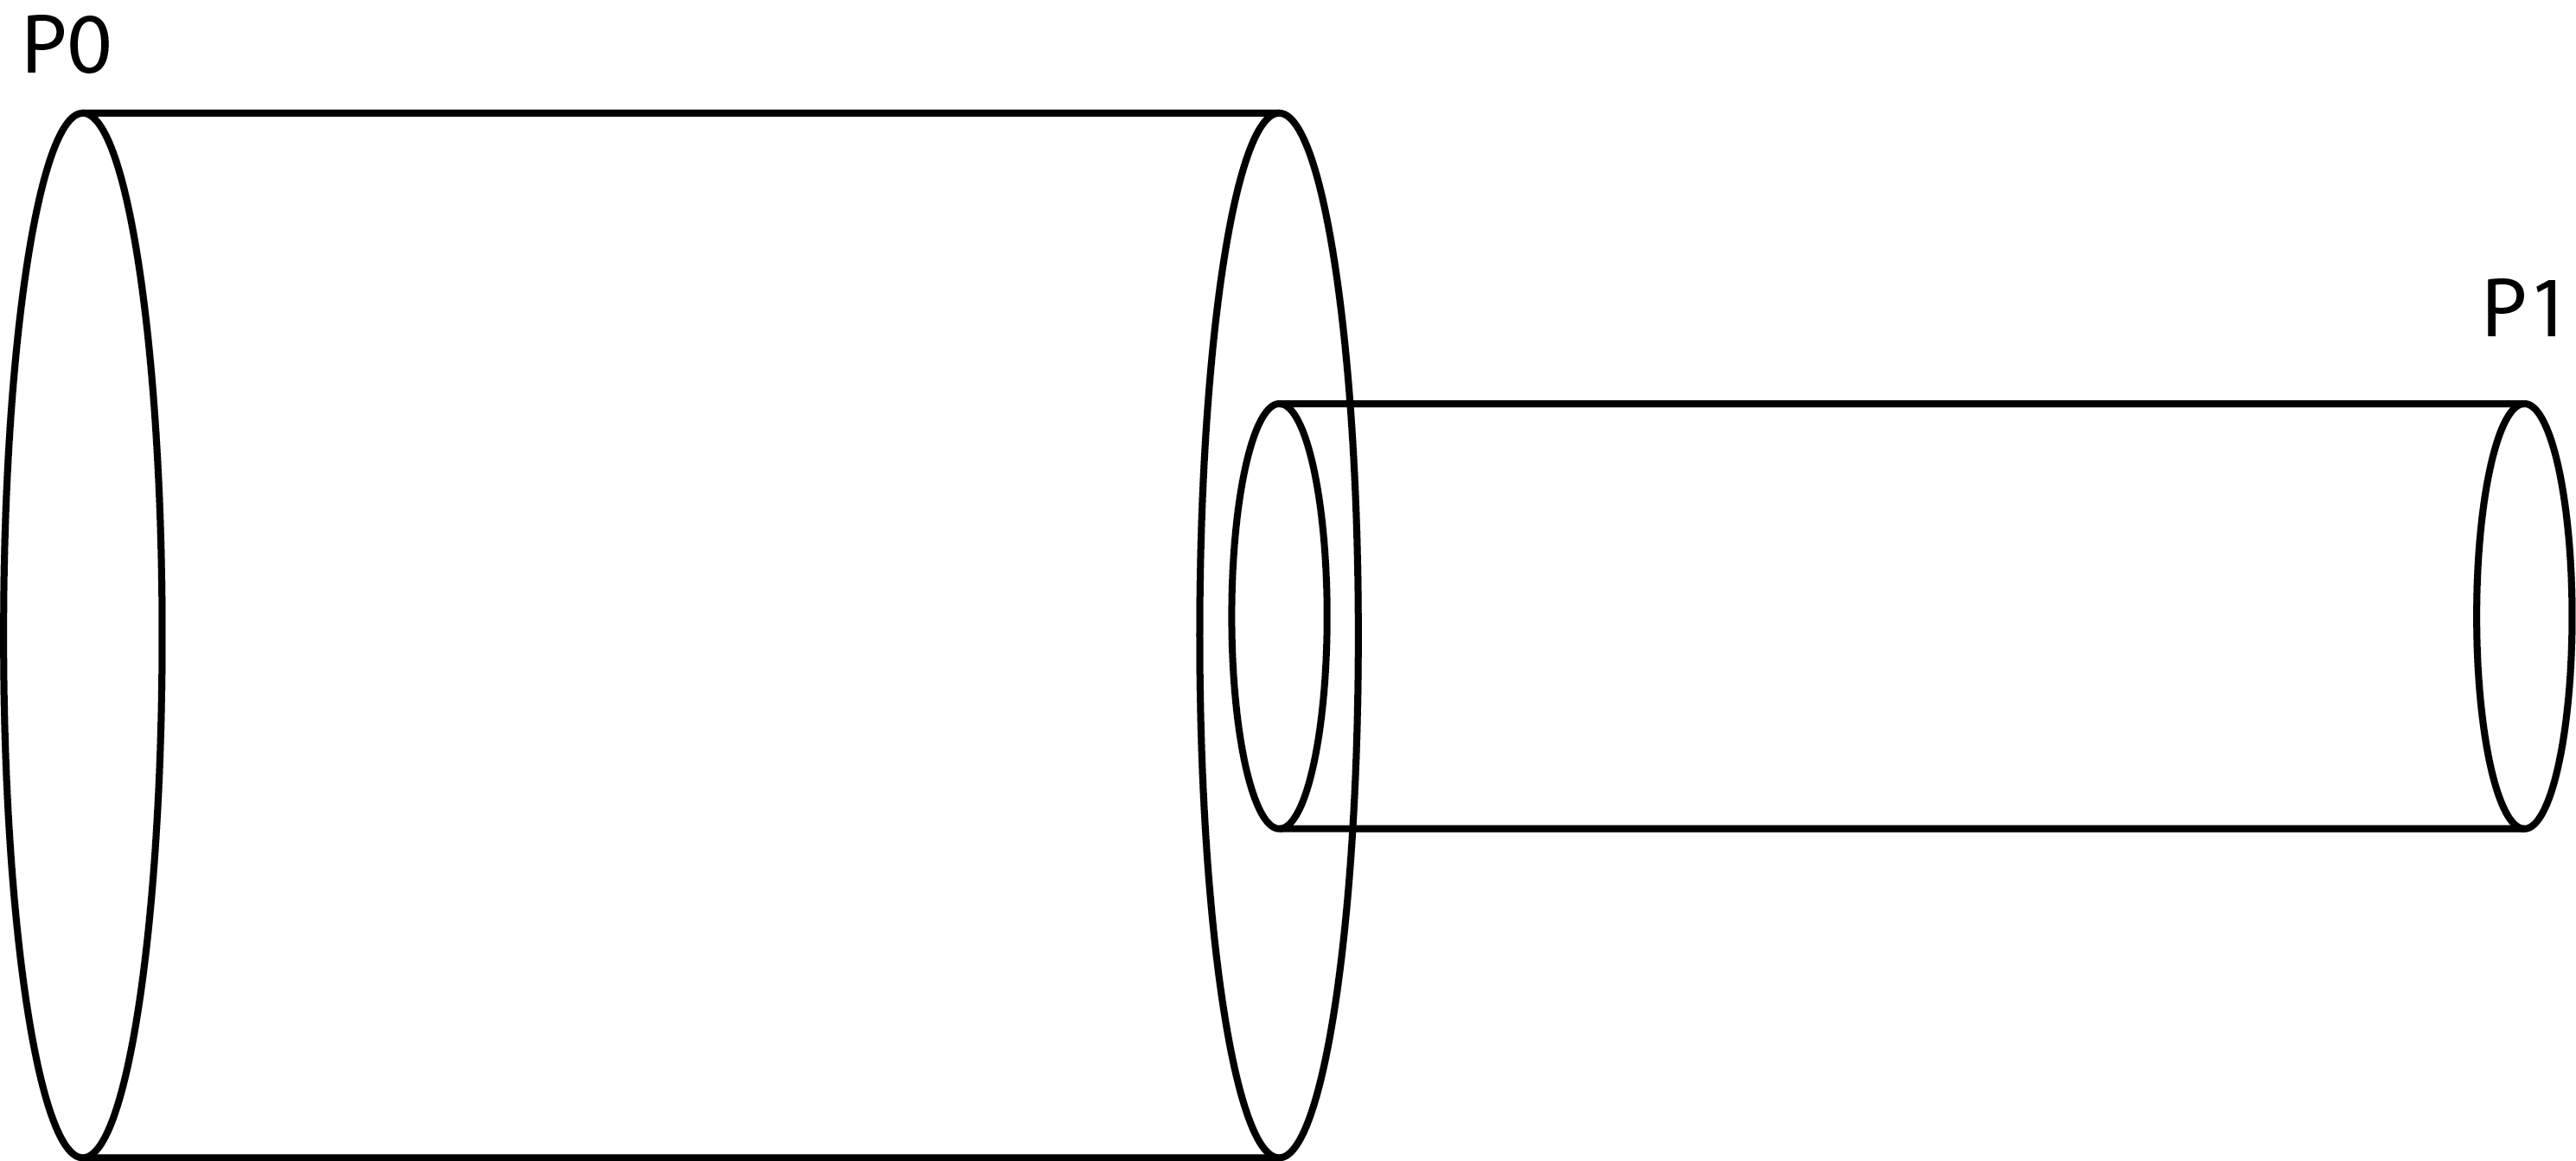
\includegraphics[width=.5\textwidth]{./Figs/twopipes}}
\caption{Two pipe model}
\label{sup-fig4}
\end{figure}  
%
The ODE set is
%
\begin{align}
  P - P_0 = R(d_1) Q \\
  P_1 - P = R(d_2) Q \\
  R(d) = \frac{c}{d^4} 
\end{align}
%
which results in the following equation
%
\begin{align}
  P_1 - P_0 = \lp R(d_1) + R(d_2) \rp Q \\
  \text{set } P_{0} = 0 \quad \to \quad P_1  =  \lp R(d_1) + R(d_2) \rp Q 
\end{align}




\section{Numerical Simulation From the paper}


\begin{figure}[h]
 \centerline{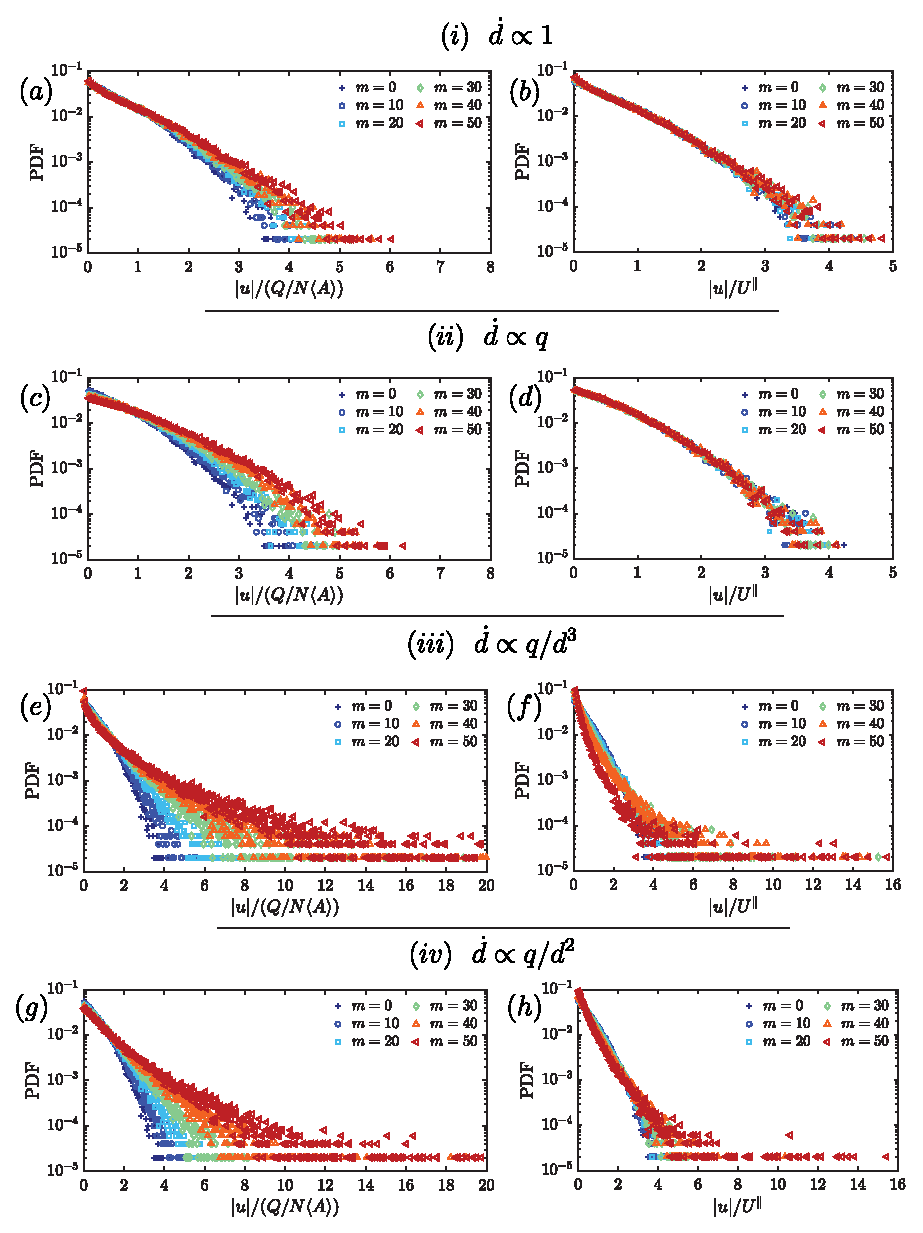
\includegraphics[width=.9\textwidth]{./Figs/pdf_combined_final.eps}}
\caption{Gradual diameter reduction of tubes (i) at a constant rate, proportional to (ii) the local flux, (iii) local shear rate at the tube's wall, (iv) local velocity. The left figures correspond to gradual changes in probability distribution of magnitude of fluid flow velocity normalized by the interstitial velocity. At each iteration the diameters are reduced as $d_\text{new} = d_\text{old}-\alpha \delta$ where $\alpha$ is a constant value such that $\langle \alpha d \rangle/\langle d\rangle = 0.02\%$. Iterations are indexed by $m$. Figures on the right correspond to the collapse of probability distribution curves when normalized by the apparent velocity $U^\parallel$ which is calculated using inverse square scaling with the measured permeability.}
\label{sup-fig4}
\end{figure}

\subsection{manuscript} 

We further develop a numerical model to examine the introduced normalization  in a random network of tubes and to obtain insights on the dynamics of local pore size changes.
% and then utilize permeability normalization
It has been shown that at low porosities $\phi<0.6$, a network of tubes with random diameters correctly captures flow behaviors of a porous medium~\cite{alim2017local}. 
% such as the exponential distribution of fluid velocity \cite{alim2017local}. 
We consider a network of tubes with a random distribution of diameters  as shown in Fig.~\ref{fig4}b. Assuming Poiseuille flow and solving for conservation of mass at all nodes, the fluid flow velocity in each tube is obtained  (see supplementary material for details). Considering different distribution of diameters (uniform, log-normal, or truncated normal) in 2D or 3D, an exponential tail for probability distribution function (PDF) of magnitude of fluid flow is observed which is in agreement with previous studies~\cite{alim2017local}. We now model a gradual polymer retention in the network of tubes with gradual reduction of tubes' diameters in iterations. We consider different diameter reduction rates: a (i) constant rate, or a rate proportional to the (ii) local flux, (iii) local shear rate, or (iv) local velocity. Among these different cases, we observe that a constant rate or a rate proportional to the local flux behaves similar to the experimental results. The gradual reduction of diameters broadens the PDF of velocity and furthermore the normalization of interstitial velocity using bulk permeability results in a decent collapse of probability distribution functions. (See Fig. \ref{fig4}c,d). In addition to the collapse of PDFs, changes in permeability, porosity, and average change of velocity are also consistent with the experimental results (see supplementary material for details). Although the numerical results closely approximate the experimental results, it should be noted that  the study here is insufficient to conclude any definite answer for the precise mechanism of diameter reduction.
% polymer retention in the tubes. 

\subsection{supplumentary}
We use our approximate numerical model as a proxy to investigate the polymer adsorption rate in the pores. We gradually reduce  tubes' diameters through iterations while we monitor changes in the distribution of fluid flow velocity and examine if such changes preserve the scaling law introduced earlier. The rate of tube's diameter reduction $\delta$, which represent the polymer deposition in the pores, can be considered (i) constant ($\delta \propto 1$), (ii) proportional to the flux rate in the tube ($\delta \propto q$), (iii) proportional to shear rate at tube's wall ($\delta \propto q/d^3$), or even (iv) proportional the the velocity in the tube ($\delta \propto q/d^2$). For each process, we pick a uniform distribution of diameters with $\langle d\rangle =10,\sigma_r=0.5$ and obtain the flow rates throughout the pipes. We then reduce the tubes diameter  $d_\text{new} = d_\text{old} - \alpha \delta $ where  $\alpha$ is a constant chosen such that the normalized average of diameter reduction be 0.2\% i.e., $\langle \alpha \delta\rangle /\langle d\rangle = 0.2\%$. After this small diameter reduction, we recalculate the flow in the tubes and reiterate the process.  Each iteration is indexed by $m$ and the result for different diameter reduction procedures are shown in Fig. \ref{sup-fig4}~a,c,e,g.
% The probability distribution for magnitude of fluid velocity  normalized by interstitial velocity remains exponential decaying consistent with experimental measurements. 
In the case of constant diameter reduction  or diameter reduction proportional to the local flux, the probability distribution for magnitude of velocity remains exponential and the tail of distribution broadens slowly (see Fig. \ref{sup-fig4}a,c). However, when diameter reduction is  proportional to shear rate or velocity, the distribution starts to diverge from an exponential and extreme large values in the tail is observed (see Fig. \ref{sup-fig4}e,g). The results for normalizing the interstitial velocity using permeability values are shown in \ref{sup-fig4}~b,d,f,h for different cases. When the diameter reduction is at a constant rate or proportional to the local flux, the scaling law is conserved (see Fig. \ref{sup-fig4}~b,d); however, when the diameter reduction is proportional to the shear rate or tube's velocity the tail of the probability distribution fails to collapse on a single curve. Based on the above numerical experiments, the dynamics of polymer retention is consistent with the models of diameter reduction either at a constant rate or at a rate proportional to the local flux. We further compare the details of changes where in the experiments we found that the permeability decreases by $60\%$, while porosity only decreases by $20\%$, and average velocity increases by $70\%$. In the case where diameter reduces proportional to the local flux, we find that after $m=55$ iterations the permeability reduces by $60\%$, while the porosity decreases by $20\%$ and average velocity increases by $67\%$; while in the case of constant diameter reduction  after $m=100$ iterations, the permeability reduces by $60\%$, the porosity decreases by $30\%$, while the average velocity increases by $50\%$. As a result, the diameter reduction proportional to the flux rate better matches with the experimental results. 





\newpage

\section{Percolation}

Percolation theory is about emergent conectivity properties of large
number of objects. The objects are extended spatially and the
positioning are statistically prescribed.






\textbf{Definition:} A cluster is a group of nearest neighboring occupied
sites.

\textbf{Definition}: The cluster number $n_s(p)$ denotes the number of
$s$-clusters per lattice site.

\textbf{Definition}: The percolation threshold $p_c$ is the
concentration (occupation probability) $p$ at which an infinite
cluster appears for the first time in an infinite lattice.

\textbf{Definition}: If $\Pi(p,L)$ denotes the probability that a
lattice of linear size $L$ percolates at concentration $L$, then
%
\begin{align}
  \lim_{L\to \infty}\Pi (p, L) =
  \begin{cases}
    0 & \text{if } p<p_c \\
    1 & \text{if } p\geq p_c
  \end{cases}
\end{align}
%


\section{Percolation in 1D}

Consider a 1d lattice of size $L$ where each site is occupied with the
probability $p$. Since the probability of occupying the sites are
independent, then the probability of all sites being occcupied is 
%
\begin{align}
  \Pi (p, L) = p^L
\end{align}
%
therefore
%
\begin{align}
  \lim_{p\to \infty} \Pi (p,L) = \lim_{L\to \infty} p^L  =
  \begin{cases}
    0 & \text{if } p <1 \\
    1 & \text{if } p =1
  \end{cases}
\end{align}
%
This implies that $p_c = 1$. 


The number of $s$-clusters can be found as
%
\begin{align}
  n_s(p) = (1-p) p^s (1-p)
\end{align}
%
This expression can be re-written as 
%
\begin{align}
  n_s(p) & = (1-p) p^s (1-p) \\
         & = (1-p)^{2} p^s  \\
         & = (1-p)^{2} \exp(s \log (p) ) \\
         & = (p_c-p)^{2} \exp(-\frac{s}{s_{\zeta}})
\end{align}
%
where
%
\begin{align}
  s_{\zeta}  = - \frac{1}{\log(p)}  = -\frac{1}{\log(p_c - (p_c - p) )} 
\end{align}
%
As a result, when $p\to p_c$, then
%
\begin{align}
  s_{\zeta } \to \frac{1}{p_{c}-p}, \qquad p \to p_c. 
\end{align}
%
Therefore the $n_s(p)$ as $p\to p_c$ becomes
%
\begin{align}
  n_s(p) & \to (p_c-p) \exp( - (p_c-p) s) 
\end{align}
%
therefore if we plot $s^2 n_s (p) $ versus $s^2 (p_c-p)$ all the
graphs should collapse on each other if $p \to p_c$. 



\textbf{Definition:} The critical exponent $\sigma $is defined as
%
\begin{align}
  s_{\zeta} \propto (p_c - p)^{\frac{1}{\sigma} }, \qquad p \to p_c
\end{align}
%

Next, we want to prove that
%
\begin{align}
  \sum_{s=1}^{\infty} s n_s(p) = p 
\end{align}
%
In the LHS, the $s n_s(p)$ is the probability that an arbitrary site
belongs to a $s$-cluster size. If we add these probabilities for all
cluster sizes, it should become the probability of the site being
occupied. To show this, we have
%
\begin{align}
  \sum_{s=1}^{\infty} s n_s(p) &= \sum _{s=1}^{\infty} s (1-p)^2 p^s \\
                               & = \sum_{s =1}^{\infty} (1-p)^2p \frac{\d}{\d p} p ^s \\
                               & = (1-p)^2 p \frac{\d }{\d p} \sum_{s = 1} ^{\infty} p^s \\
                               & = (1-p)^2 p \frac{\d }{\d p } \frac{p}{1-p} \\
  & = p.
\end{align}
%


The next question is, how large on average clusters are? At first, we
need to see what is the probability of a cluster with size $s$? We
know that the probability of a site belonging to a cluster size $s$ is
$sn_s(p)$, and the probability of that point belongs to any cluster
size is $p$. Therefore each point has the probability of $w_s = s n_s(p)/p$
belonging to a cluster size $s$ among all clusters. Therefore
%
\begin{align}
  w_s = \frac{s n_{s}(p)}{p} = \frac{ s n_{s}(p) }{ \sum_{s=1}^{\infty} s n_{s}(p)} 
\end{align}
%
Now, we can calculate the mean cluster size as
%
\begin{align}
  S(p) & = \sum_{s=1}^{\infty} s w_s(p) = \frac{\sum_{s=1}^{\infty} s^2 n_s(p) }{\sum s n_s(p) }   \\
       & = \frac{1}{p} (1-p)^2 (p \frac{\d}{\d p} ) (p \frac{\d }{\d p } ) \sum_{s=1}^{\infty} p^{s}\\
  & = \frac{1+p}{1-p} 
\end{align}



\textbf{Definition}: The correlation funtion or pair conectivity
$g(r)$ is the probability that a site at position $r$ from an occupied
site belongs to the same finite cluster. Note that clearly $g(r= 0) =
1$ since the site is already occupied. 


In 1D, the correlation function is calculated as
%
\begin{align}
  g(r) = p \cdot p \cdot \cdots \cdot p =   p^r
\end{align}
%
We normally express this in an exponential form and find the critical
exponent as
%
\begin{align}
  & g(r) = p^r = \exp (r \log(p)) = \exp (-\frac{r}{\zeta})\\
  & \zeta = -\frac{1}{\log (p) } = -\frac{1}{\log\lb p_c - (p_c-p)\rb} \to (p_c-p)^{-1}, \quad p\to p_c  
\end{align}
%
The value of $\zeta$ is known as correlation length which diverges as
$p\to p_c$. In 1D, we found that $\zeta = s_{\zeta}$, where it is not
normally true; normally $s_{\zeta} \propto \zeta^D$ where $D$ is the
fractal dimention.

\textbf{Definition}: The critical exponent $\nu$ is defined by
%
\begin{align}
  \zeta \propto |p_c-p|^{\nu}, \qquad p \to p_c
\end{align}
%

??????? I don't know why, but it is aruged that
%
\begin{align}
  \sum_r g(r) = S(p) 
\end{align}



\section{Infinite Dimension}

Percolation in 1D and infinite dimension can be solved
analytically. The infinte dimension is similar to the Beth lattice.

\subsection{Beth Lattice}

In Beth lattice, each site (vortex) is connected to $z$ neighbors
(vortices). As a result each branch (edge) is connected to $z-1$ other
branches.

\begin{figure}[h]
  \centering
  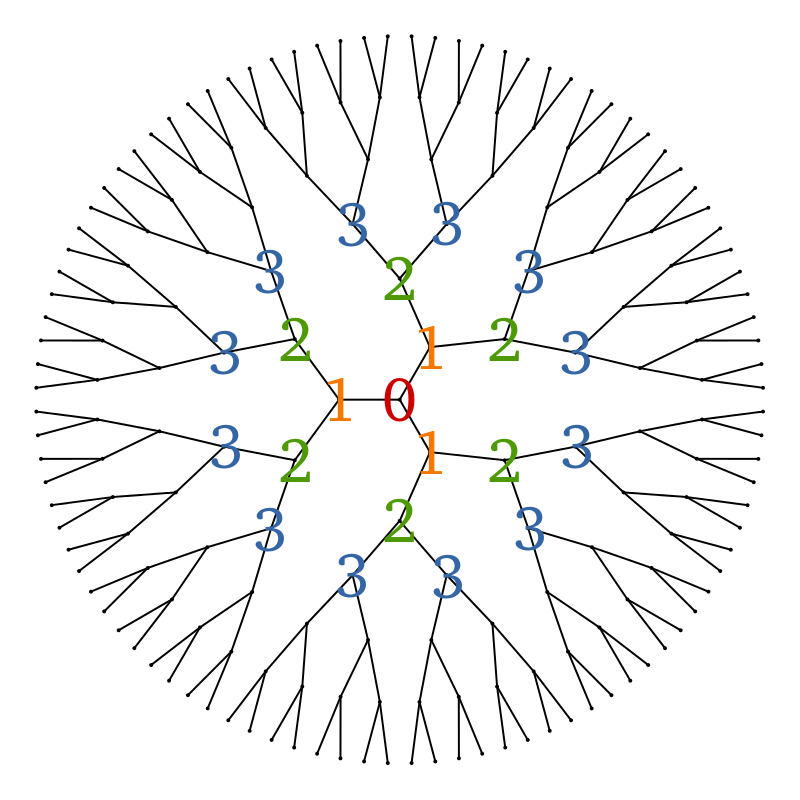
\includegraphics[width=8cm]{beth-lattice}
  \caption{Beth Lattice with $z=3$. Source: wikipedia}
\end{figure}

The 1D case that we studied is essentially a Beth lattice with
$z=2$. The next question is why Beth lattice corresponds to $d=
\infty$? The reasons are

\begin{itemize}
\item (a) The number of surface sites relative to total number of
  sites approaches a constant as $d\to \infty$.

  The total number of sites in Beth lattice are number of sites from
  generation 0 plus number of sites in generation 1 added
  together. Assume we have a Beth lattice with $z=3$, and we go upto
  $g$ generations then
%
\begin{align}
  \text{total number of sites } & = 1 + 3 + 3\cdot 2 + 3 \cdot 2^2 + \cdots + 3 \cdot 2^{g-1} \\
                                & = 1 + 3(1 + 2 + 2^2 + 2^3 + \cdots + 2^{g-1}) \\
  & = 1 + 3 \frac{2^{g}-1 }{2-1}  = 3\cdot 2^g -2 
\end{align}
%
while the total number of surface sites (sites at the outer most
boundary) are $3\cdot 2^{g-1}$. Therefore
%
\begin{align}
  \frac{\text{Number of surface sites}}{\text{Total Num of sites}} = \frac{3\cdot 2^{g-1}}{3 \cdot 2^{g} - 2} \to \frac{1}{2}, \qquad g\to \infty  
\end{align}

Generally, the numbers are a s
%
\begin{align}
  \text{total number of sites} & = 1 + z (1 + (z-1) + (z-1)^{2} + \cdots + (z-1)^{g-1}) \\
  & = 1  + z \frac{(z-1)^{g} - 1 }{z - 2} 
\end{align}
%
therefore
%
\begin{align}
  \frac{\text{Number of surface sites}}{\text{Total Num of sites}} &= \frac{ z \cdot (z-1)^{g-1}}{1  + z \frac{(z-1)^{g} - 1 }{z - 2} } \\
                                                                   & =  \frac{(z-1)^g + (z-1)^{g-1}}{ \frac{z-2 + (z-1)^{g+1} + (z-1)^g - z }{z-2}  }  \\
                                                                   & \to  \frac{(z-2)(z-1)^g}{(z-1)^{g+1}} = \frac{z-2}{z-1} 
\end{align}


In a hypercube lattice of linear size $L$ when $d\to \infty$, the
surface in a $d$ dimension is proportional to $L^{d-1}$ and the volume
is proportional to $L^d$, therefore
%
\begin{align}
  \text{Surface} \propto \text{Volume}^{\frac{d-1}{d}}  = \text{Volume}^{1 - \frac{1}{d}}
\end{align}
%
therefore as $d\to \infty$, the ration of the surface to volume
becomes a constant. 



\item (b) There are no closed loops in Bethe lattice. In a hypercube
  lattice the probability of finding a close loop is zero. Assume a
  $d$ dimension hypercube and a particle centered at a site. There are
  $2d$ nearest sites that the next particle can be placed. The next
  particles can be placed at $2d-1$ positions. Therefore assuming a 4
  point lattice, there are $2d (2d-1)^2$ possibilities. If now we want
  to put these 4 points in a lattice, we have $2d$ for the second
  particle, $2d-2$ positions for the third particle and only $1$
  position for the last particle. Therefore
  %
  \begin{align}
    \frac{\text{Number of loops}}{\text{Total number of chains}} = \frac{2d\cdot(2d-2)\cdot 1 }{2d (2d-1)^{2}}   \to 0, \qquad d\to \infty
  \end{align}
  
\end{itemize}

For these two reasons, a Bethe lattice is considered as infinite
dimension lattice.

\textbf{Question}. What is the occupation probability to make sure an
infinite path occurs in a Bethe lattice? Starting from the center,
there are $z-1$ neighbors, and assuming an occupation probability of
$p$, we have $p(z-1)$ occupied sites. We need to make sure that at
least one occupied site exists, therefore
%
\begin{align}
  p_c(z-1) = 1 \to p_c = \frac{1}{z-1} 
\end{align}
%


\textbf{Definition}: The strength of an infinite cluster $P(p)$ is the
probability that an arbitrary site belongs to an infinite cluster. 




\section{Random Walk}

\subsection{Random Walk and Diffusion Equation}


If at time $t$ the probability distribution is as
$p(\mathbf{r},t)$. Now assume $\tau$ time later, we need to integrate
over all the space. We have
%
\begin{align}
  p(\mathbf{r},t + \tau ) = \int p(\mathbf{r}- \mathbf{l}, t) g(\mathbf{l}) \d \mathbf{l} 
\end{align}
%
To proceed we do the Taylor expansion, we find that
%
\begin{align}
  p(\mathbf{r}-\mathbf{l},t) \approx p(\mathbf{r},t) - \n p \cdot \mathbf{l} + \frac{1}{2}  \sum_{ij} \frac{\p^{2} p}{\p x_i \p x_j} l_i l_j \\
  p(\mathbf{r}, t+\tau) = p(\mathbf{r},t) + \tau \frac{\p p }{\p t} 
\end{align}
%
Therefore,
%
\begin{align}
  & p(\mathbf{r},t) + \tau \frac{\p p }{\p t}   = \nonumber \\
  & \qquad  \int \lb p(\mathbf{r},t) - \n p \cdot \mathbf{l} + \frac{1}{2}  \sum_{ij} \frac{\p^{2} p}{\p x_i \p x_j} l_i l_j \rb g(\mathbf{l}) \d \mathbf{l} \\
   & p(\mathbf{r},t) + \tau \frac{\p p }{\p t}   = \nonumber \\
  & \qquad   p (\mathbf{r},t) - \n p \cdot \int \mathbf{l}  g(\mathbf{l}) \d \mathbf{l} +  \int \frac{1}{2}  \sum_{ij} \frac{\p^{2} p}{\p x_i \p x_j} l_i l_j g(\mathbf{l}) \d \mathbf{l} 
\end{align}
%
If the diffusion process is isotropic, then there is no difference
between $\pm \mathbf{l}$, therefore the second term on the RHS
vanishes as
%
\begin{align}
  \int \mathbf{l} g(\mathbf{l}) \d \mathbf{l} = 0  
\end{align}
%
The relation therfore summarizes to
%
\begin{align}
  \tau \frac{\p p }{\p t}  = \frac{1}{2} \int \sum_{ij} \frac{\p^{2} p }{\p x_i \p x_j} l_il_j g(\mathbf{l}) \d \mathbf{l} 
\end{align}
%
If we assume that the diffusion is isotropic, i.e., $g(x,y,z) =
g(-x,y,z)$ and etc., then only the diagonal terms survive and we obtain
%
\begin{align}
  \tau \frac{\p p }{\p t}  = \frac{1}{2} \int \sum_{i} \frac{\p^{2} p }{\p x_i \p x_i} l_i^2 g(\mathbf{l}) \d \mathbf{l} \\
    \tau \frac{\p p }{\p t}  = \frac{1}{2} \sum_{i} \frac{\p^{2} p }{\p x_i \p x_i} \int  l_i^2 g(\mathbf{l}) \d \mathbf{l} 
\end{align}
%
We furthermore have that
%
\begin{align}
  \int l_i^2 g(\mathbf{l}) d \mathbf{l} = \frac{1}{3} \int \mathbf{l}\cdot \mathbf{l} g(\mathbf{l}) d \mathbf{l} = < \mathbf{l}^2>
\end{align}
%
Therefore, we finally obtain
%

\begin{align}
  \tau \frac{\p p }{\p t}  = \frac{1}{6} \n^2p < \mathbf{l}^2> \\
  \frac{\p p }{\p t}  = \frac{<\mathbf{l}^2>}{6\tau} \n^2p 
\end{align}
%
where we can summarize the final equation as
%
\begin{align}
  \frac{\p p}{\p \tau}  = D \n^2p
\end{align}
%
in which $D =  <\mathbf{l}^2> / 6\tau$ is the diffusion constant. 



\subsection{Normal Diffusion}

There are various approaches to the diffusion equation. 
\subsubsection{Fick's law}
%
Diffusion was pioneered by Fick motivated by a biological application
(transport through membranes). By conservation law for total number of
particles, he derived the diffusion equtaion for concentration of
species as
%
\begin{align}
  \frac{\p c}{\p t} = D \frac{\p^{2} c}{\p x^2}  
\end{align}
%
The derivation is as follows: Assume we have $N(x)$ particles at
position $x$, and $N(x + \Delta x) $ at position $x+\Delta x$. The
cross section area in between these points is $A$. The question is how
many particles will pass through this cross sectional area. Half of
the particles at $x$ move to right and the other half to the
left. Same story for the particles at $x + \Delta x$. Therefore the
flux of molecules $J$ through the area $A$ during a short time $\tau$
is
%
\begin{align}
  J = \frac{ -\frac{1}{2} ( N(x+ \Delta x) - N(x)  }{A \tau} 
\end{align}
%
we define concentration $c \equiv {N(x) }/ {A \Delta x} $, therefore
the flux becomes
%
\begin{align}
  J = - \frac{\Delta x ^{2}}{2 \tau} \frac{ c(x + \Delta x) - c(x) }{\Delta x} = - D \frac{\p c }{\p x }  
\end{align}
%
therefore the flux is proportional to the diffusion constant $D \equiv
\Delta x ^2/2 \tau$ and the gradient of concentration.
%
Since the total number of particles are conserved, then
%
\begin{align}
  \frac{c(t+\Delta t) - c(t)}{\Delta t} = \frac{1}{\Delta t} \frac{\lp J(x) - J(x+\Delta x)\rp A\Delta t }{A \Delta x} =   - \frac{ J(x+\Delta x) - J(x) }{ \Delta x} 
\end{align}
%
Therefore the results summarizes to
%
\begin{align}
  \frac{\p c}{\p t}  = - \frac{\p J]}{\p t}, \qquad J = -D \frac{\p c}{\p x} 
\end{align}
%
or in one diffusion equation as
%
\begin{align}
  \frac{\p c}{\p t}  = D \frac{\p ^{2}c }{\p t^2} 
\end{align}
%

%
\textbf{Observations}:
%
\begin{itemize}
\item The same equation holds for the probability density (PDF)
  $p(x,t)$ to find a particle at position $x$ and time $t$
\item The PDF of the position of particles starting from a
  concentrated droplet in an unbounded medium is Gaussian with
  variance $2Dt$
\item It means that the particles mean squared displacement (MSD) in
  the $x$-direction grows proportionally with time $<x^2> = 2Dt$,
  where the coefficient of this proportionality is twice the diffusion
  constant $D$
\item The same is true for other coordinates, so the toal MSD grows as
  $<r^2> = 2dD t$, where $d$ is the dimension of the space. 
\end{itemize}






\subsubsection{Microscopic, molecular approach}

Done by Einstein! It is essentially a random walk. It samples
particles at discrete istant of time separated by interval $\tau$. How
does the known MSD behavior in diffusion emerges from such a model?

Assume the particle is taking steps $s_i$ at each time. The particle's
displacement is then given by
%
\begin{align}
  x(t) = \sum_1^{N(t)} s_i
\end{align}
%
where $N(t)$ is the total number of steps performed until time
$t$. From this picture, we get
%
\begin{align}
  \langle x(t)^2 \rangle= \la \lp \sum_1^{N(t)} s_i \rp^{2} \ra = \la \sum_{i,j = 1}^{N(t)} s_i s_j \ra = \la \sum_{i =1}^{N(t)} s_i^2 \ra + \la \sum_{i\neq j} s_i s_j\ra 
\end{align}
%
So the MSD is expressable through step correlation function $C_{ij} =
\la s_i s_{j }\ra $. Since the steps are assumed to be independent and
uncorrelated and symmetrically distributed around zero, the last term
vanishes . The mean squared displacement of each step is $\la s_i^2
\ra  = a^2$, thus
%
\begin{align}
  \la x(t) ^2 \ra = \sum_{i=1}^{N(t)} \la s_i^2\ra  = N(t) a^2 = \frac{a^{2}}{\tau} t
\end{align}
%
So the diffusion coefficient becomes as $D = a^2/2\tau$. The term $k
\equiv 1/\tau$ is the rate of steps or the mean number of steps per
unit time.


\subsubsection{Langevin Approach}

In this approach, paqrticles are moving in a fluid medium following
Newtonian Mechanics and under the influence of esxternal forces and
friction! The effect of thermal motion of the molecules and of the
surrounding medium are modeled with addisional random force term
(``noise''). The equation of motion is then
%
\begin{align}
  m\dot v = - \gamma v + f + \zeta (t) \label{eq-langevin}
\end{align}
%
where $m$ is the mass, $\gamma$ is the friction, and $\zeta$ is the
random force, and $f$ is the external force. From this equation
Langevin was able to derive MSD of the particles.


In order to solve the \eqref{eq-langevin} equation, lets first assume
there is no external force and no randomness. Therefore, the equation
is dominated by the viscous force and we have
%
\begin{align}
  m \dot v = -\gamma v
\end{align}
%
where the solution is
%
\begin{align}
  v(t) = \exp(-\gamma t /m) v(0)
\end{align}
%
which means that the velocity vanishes. We know that the average of
random particles should become $1/2 m \la v^2 \ra = 1/2 k_BT$, so the
particles are not only derived by the viscous term. Lets add the
random force, we have
%
\begin{align}
  m\dot v = - \gamma v + \zeta (t) 
\end{align}
%
Now that we have $\zeta (t)$ on the right hand side, we assume the
solution to have the following form
%
\begin{align}
  v(t) = e^{- \gamma t /m } b(t)
\end{align}
%
replacing back in the governing equation, we obtian
%
\begin{align}
  \dot b (t) = e^{\gamma t/m}\zeta (t) /m 
\end{align}
%
Note that the initial condition for $b(0) = v(0)$. The solution of $b(t)$ becomes as
%
\begin{align}
  b(t) = v(0) + \int_0^t e^{\gamma  s/m} \zeta(s) /m ~\d s 
\end{align}
%
putting everything together, the solution becomes as
%
\begin{align}
  v(t) =  e^{- \gamma/m t} v(0) + \int_0^t  e^{- \gamma (t-s)/m} \zeta (s) /m ~ \d s 
\end{align}
%
Now lets calculate the mean squared velocity, we have
%
\begin{align}
  \la v(t) \ra ^2 =  \la e^{- 2\gamma/m t} v(0)^2 \ra + 2 \la e^{- \gamma/m t} v(0)\cdot \int_0^t   e^{- \gamma (t-s)/m} \zeta (s) /m ~ \d s \ra + \la \int_0^t  \lp e^{- \gamma (t-s)/m} \zeta (s) /m ~ \d s\rp ^2 \ra
\end{align}
%
If we assume that $\la \zeta \ra = 0$, and $\la \zeta (t) \zeta (s)
\ra = 2 B \delta (t-s)  $, therefore the result become as
%
\begin{align}
  \la v(t)^{2} \ra & = \la e^{- 2\gamma/m t} v(0)^2 \ra + \int_0^t \int _0^t  e^{- \gamma (t-s)/m} e^{- \gamma (t-s')/m} \frac{ \la \zeta (s) \zeta (s') \ra}{m^2} ~ \d s ~ \d s' ~  \\
                  & = \la e^{- 2\gamma/m t} v(0)^2 \ra + \int_0^t \int _0^t  e^{- \gamma (t-s)/m} e^{- \gamma (t-s')/m} \frac{ 2 B \delta (s-s') }{m^2} ~ \d s ~ \d s' ~ \\
                  & = \la e^{- 2\gamma/m t} v(0)^2 \ra +  \int_0^t   e^{- 2\gamma (t-s)/m} \frac{ 2 B }{m^2} ~ \d s \\
  &  = e^{- 2\gamma/m t} v(0)^2  + \frac{B}{\gamma m} \lp 1 - e^{-2\gamma t/m }\rp
\end{align}













\subsection{1D - Random Walk - Characteristic Function}
%
In 1d random walk we have the following
%
\begin{align}
  x =
  \begin{cases}
    1, & \text{probability  } p \\
    -1 & \text{probability  } q
  \end{cases}
\end{align}
%
we define the characteristic function $\lambda(\th) = \la e^{i \theta x} \ra
$.  Therefore, 
% 
\begin{align}
  \lambda = p e^{i\theta} + q e^{-i\theta}
\end{align}
%
We can now find the probability of the object being at $j$th location
after $n$ steps by calculating the coefient of
%
\begin{align}
  P_n(j) = \frac{1}{2\pi} \int_{-\pi}^{\pi} \lp p e^{i\theta} + q e^{-i\theta} \rp^n e^{-ij\th}\d \th
\end{align}
%
which is giving out the coefficient corresponding to the $j$th
position. Noting that
%
\begin{align}
  \frac{1}{2\pi} \int_{-\pi}^{\pi} e^{-i\th n}\d \th = \delta_{n,0}
\end{align}
%
one can calculate the above expression. In the case of $p=q = 1/2$,
the expression reduces to
%
\begin{align}
  \lambda (\th) = \cos(\th). \to P_n(j) = \frac{1}{2\pi} \int_{-\pi}^{\pi} \cos\th^n e^{-ij \th}\d \th
\end{align}

\subsubsection{General case}

Assume the random walker picks its displacement per step by a
probability density function $p(x)$. 





\newpage

\section{Poroelasticity}

The coupling between changes in stress and changes in fluid pressure
forms the subject of poroelasticity


There are two types of coupling:
%
\begin{itemize}
  \item Solid-to-Fluid Coupling: a change in applied stress produces a
    change in the fluid pressure. The magnitude of this coupling
    depends on the compressibility of the fluid. 
  \item Fluid-to-solid Coupling: A change in Fluid pressure changes the volume of porous material
\end{itemize}
%

Assumptions and terms usually used:
%
\begin{itemize}
\item fluid pressure and pore pressure are usually used
  interchangeably
 \item elastic wave propagation due to fluid-solid interaction is also
   usually ignored
\end{itemize}


\begin{itemize}
\item Poroelastic equations were derived by Biot
  \cite[][]{biot_general_1941,biot_theory_1955,biot_theory_1956}

  A review of Biot's approach is as follows:
  \begin{itemize}
  \item $\sigma$: isotropic applied stress, positive if tensile,
    negative if compressive
   \item $V$: the bulk volume
   \item $\ep = \delta V/V$ volumetric strain, positive in expansion,
     negative in contraction
   \item $\zeta$ increment in fluid content
   \item $p$ fluid pressure
   \end{itemize}
   Constitutive relations are
   %
   \begin{align}
     \ep &= a_{11} \sigma + a_{12} p \\
     \zeta &= a_{21} \sigma + a_{22} p 
   \end{align}
\end{itemize}


\begin{figure}[h]
  \centering
  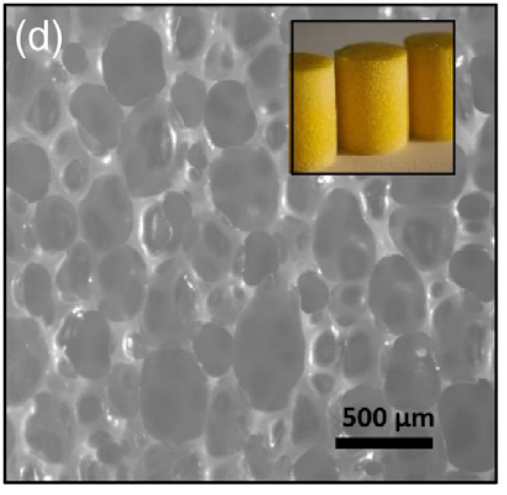
\includegraphics[width=5cm]{Figs/poroelasticity-crumble}
  \caption{Example of a 2D structure considered for percolation
    problem, Lahini \textit{et al.}, PRL, 2017 } \label{fig-soft-hard}
\end{figure}


\subsection{Mandel Cryer Effect}


Model is as follows:
%
\begin{align}
  \sigma - \sigma_0 = \mathbf{C}: \lp \ep - \ep_0\rp - \alpha p \mathbf{I}\\
  \rho S \frac{\p p}{\p t} + \n . (\rho \mathbf{q}) = Q - \rho \a \frac{\p \ep_{v}}{\p t}\\
  \mathbf{q} = - \frac{k}{\mu} \n p 
\end{align}
%
where $\mathbf{C}$ is the stiffness tensor, $\sigma$ is the stress
tensor, $\ep$ is the strain tensor, $\rho$ is fluid density, $k$ is permeability, $\mu$ is fluid
viscosity, $S$ is the storage parameter, $\a$ is the Biot constant,
and $\ep_v$ is the volumetric strain.


\begin{figure}[h]
  \centering
  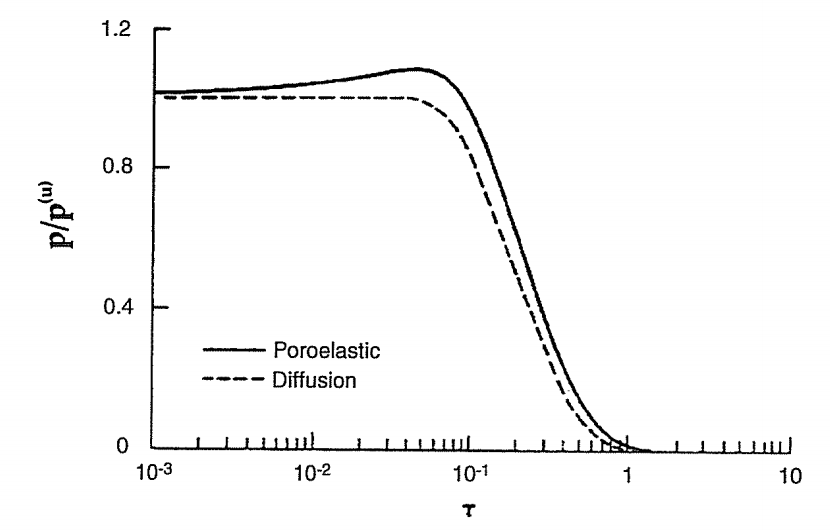
\includegraphics[width=15cm]{Figs/mandel-cryer-effect}
  \caption{Mandel-Cryer effect. Pore pressure versus time at the
    center of a poro-elastic cylinder. From p. 196, Herbert Wang, Theory of
    linear poroelasticity.} \label{fig-soft-hard}
\end{figure}





\newpage

\newpage


\section{Percolation and Structural Mechanics}

Assume we have a structure made of soft and hard materials on a 2D
lattice (see Fig. \ref{fig-soft-hard}). The proability of a site being
occupied as soft material is $p$ and the probability of the site being
occupied with hard material is $1-p$. The question is how does the
material property changes for different values of $p$? Obviously when
$p=1$, all the material is made of a soft material with its properties
and when $p=0$ the material is made of a hard material and its
properties is determined with the hard material. 

\begin{figure}[h]
  \centering
  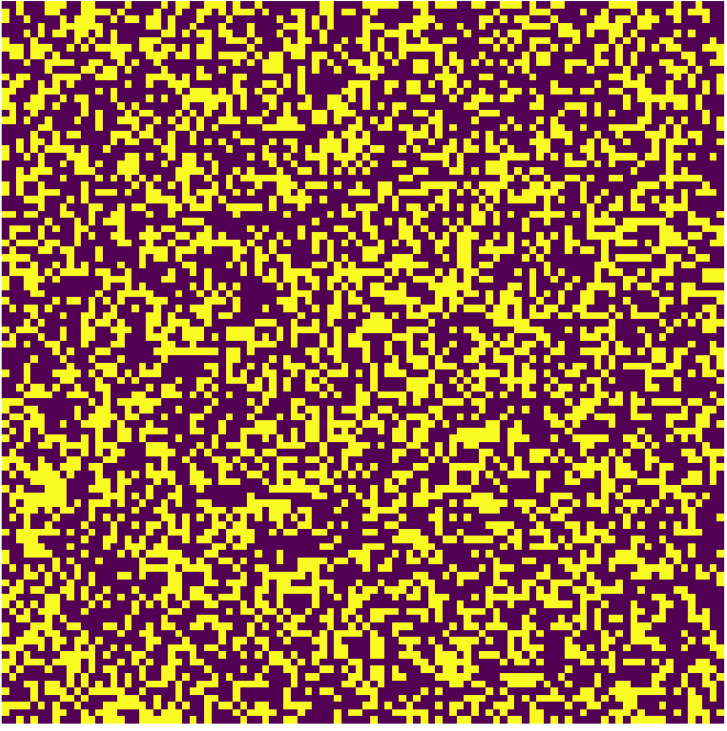
\includegraphics[width=5cm]{Figs/percolation-first}
  \caption{A 2D material with soft (yellow) and hard (black) material
    next to each other.} \label{fig-soft-hard}
\end{figure}


I would expect that the Elasticity of the 2D material have some sort
of transition from soft to hard that depends on the probability $p$. 

\begin{figure}[h]
  \centering
  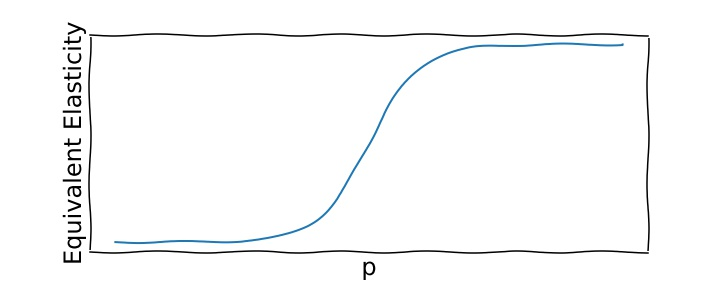
\includegraphics[width=10cm]{Figs/elasticity-percolation}
  \caption{Behavior of elasticity with percolation probability $p$} \label{fig-elasticity-percolation}
\end{figure}



\section{Elasticity}

Under action of a force, solid objects deform. Assuming a point in
solid at $\mathbf{x} = (x,y,z)$ will come to $\mathbf{X} =
(X,Y,Z)$. The vector $\mathbf{u} = \mathbf{x}- \mathbf{X}$ is then
known as displacement field. When the solid is elastic and the
displacement is small, the relation ship between stress $\sigma$, and
the strain tensor $\epsilon$ is given by Hooke's law as
%
\begin{align}
  \sigma_{ij} = \lambda \delta _{ij} \n . \mathbf{u} + 2\mu \epsilon _{ij} (\mathbf{u}) 
\end{align}
%
where the strain tensor is given as
%
\begin{align}
  \epsilon_{ij} (\mathbf{u}) = \frac{1}{2} \lp \frac{\p u_{i}}{\p x_{j}} + \frac{\p u_{j}}{\p x_{i}} \rp
\end{align}
%
The parameters $\lambda$ and $\mu$ are two constants (known as Lam\'e constants) that depend on
the material properties. 


\textbf{Question}. How does Lam\'e constants relate to the famous
Yong and shear modul of elasticity $E, G$?

We define $\varepsilon_{ij} = \p u_i/ \p x_j$. Expanding the relation
we had, we see
%
\begin{align}
  \sigma_{11} & = \lambda (\vep_{11} + \vep_{22} + \vep_{33}) + \mu \lp \vep_{11} + \vep_{11}\rp \nonumber\\
             & = ( \lambda + 2\mu )\vep_{11}  + \lambda \vep_{22} + \lambda \vep_{33} \\
  \sigma_{12} & =  \mu ( \vep _{12} + \vep _{21}) \nonumber\\
             & = 2\mu \vep_{12} 
\end{align}
%
On the other hand, by the definition of Yong modulus $E$ and shear
modulus $G$ we have
%
\begin{align}
  \vep_{11} & = \frac{1}{E}  \lb \sigma_{11} - \nu \lp \sigma_{22} + \sigma_{33}\rp \rb \\
  \vep_{22} & = \frac{1}{E}  \lb \sigma_{22} - \nu \lp \sigma_{11} + \sigma_{33}\rp \rb \\
  \vep_{33} & = \frac{1}{E}  \lb \sigma_{33} - \nu \lp \sigma_{11} + \sigma_{22}\rp \rb \\
  \vep_{12} = \frac{\sigma_{12}}{2G}, & \qquad \vep_{23} = \frac{\sigma_{23}}{2G},  \qquad \vep_{13} = \frac{\sigma_{13}}{2G}
\end{align}
%
Comparing these two set of equations, one can find that
%
\begin{align}
 \mu = G \equiv \frac{E}{2(1+\nu)} , \qquad \lambda  = \frac{E\nu}{(1-2\nu)(1+\nu)} 
\end{align}
%
\section{Equilibrium Equation - Variational Format}
%
The equilibrium equation reads as
%
\begin{align}
  \frac{\p \sigma_{ij}}{\p x_{j}}  + F_i = \ddot u_i \to \frac{\p \sigma_{ij}}{\p x_{j}}  + F_i  = 0
\end{align}
%
where the second equation is assuming the static
equilibrium. Therefore the equation that we are solving is as
%
\begin{align}
   \n \cdot \sigma + \mathbf{F} =0
\end{align}
%
To get the variational form, we multiply both sides by a test function
and integrate over a test domain $\Omega$ to obtain
%
\begin{align}
  \int_{\Omega} \lp \n \cdot\sigma\rp \cdot ~\mathbf{v} ~\d x + \int_{\Omega} \mathbf{F} \cdot \mathbf{v} ~\d x = 0\\
  \int_{\partial \Omega} (\sigma \mathbf{n})\cdot \mathbf{v} ~\d s - \int_{\Omega} \sigma : \n \mathbf{v}~ \d x + \int_{\Omega} \mathbf{F} \cdot \mathbf{v} ~\d x = 0 \label{variational-equil}
\end{align}
%
Note that in the above equations we used the following divergence
identity from vector calculus: For an arbitrary domain $D$, tensor
$A_{ij}$ and vector $b_i$, the following identity holds
%
\begin{align}
  \int_D (\n \cdot \mathbf{A}) \cdot \mathbf{b} ~ \d x  = \int_{\p D} (\mathbf{An})\cdot \mathbf{b} ~\d s  - \int_D \mathbf{A}:\n \mathbf{v} ~\d x
\end{align}
%
where $\mathbf{n}$ is the normal vector to the boundary $\p D$ and $:$
denotes the double dot product as
%
\begin{align}
  \mathbf{X}: \mathbf{Y} = \sum_{ij} X_{ij}Y_{ij}
\end{align}
%
and the gradient of the vector defined as
%
\begin{align}
  \lp \n \mathbf{v} \rp_{ij} = \frac{\p v_{i}}{\p x_{j}} 
\end{align}
%
Now getting back to equation \eqref{variational-equil}, since stress
tensor is symmetric we have
%
\begin{align}
  \int_{\partial \Omega} (\sigma \mathbf{n})\cdot \mathbf{v} ~\d s - \int_{\Omega} \sigma : \n \mathbf{v}~ \d x + \int_{\Omega} \mathbf{F} \cdot \mathbf{v} ~\d x = 0 \\
  \int_{\partial \Omega} (\sigma \mathbf{n})\cdot \mathbf{v} ~\d s - \int_{\Omega} \sigma : \frac{1}{2} \lp \n \mathbf{v} + \n \mathbf{v}^{\top} \rp ~ \d x + \int_{\Omega} \mathbf{F} \cdot \mathbf{v} ~\d x = 0 \\
    \int_{\partial \Omega} (\sigma \mathbf{n})\cdot \mathbf{v} ~\d s - \int_{\Omega} \sigma : \ep(\mathbf{v}) ~ \d x + \int_{\Omega} \mathbf{F} \cdot \mathbf{v} ~\d x = 0
\end{align}
%
From the previous section we know that
%
\begin{align}
  \sigma_{ij} = \lambda \delta _{ij} \n . \mathbf{u} + 2\mu \epsilon _{ij} (\mathbf{u}) 
\end{align}
%
Using the above equation we obtain the following variational form
%
\begin{align}
      \int_{\partial \Omega} (\sigma \mathbf{n})\cdot \mathbf{v} ~\d s - \int_{\Omega} \lambda \n \cdot \mathbf{u} \n \cdot \mathbf{v} ~ \d x  - \int 2\mu \ep (\mathbf{u}) : \ep (\mathbf{v}) ~ \d x+ \int_{\Omega} \mathbf{F} \cdot \mathbf{v} ~\d x = 0
\end{align}
%
where the first equation is usually handled with the boundary
conditions. So, we solve the following variational form equation
%
\begin{align}
  & \int_{\Omega} \lambda \n \cdot \mathbf{u} \n \cdot \mathbf{v} ~ \d x  + \int 2\mu \ep (\mathbf{u}) : \ep (\mathbf{v}) ~ \d x - \int_{\Omega} \mathbf{F} \cdot \mathbf{v} ~\d x = 0\\
  & \text{subject to } \sigma \mathbf{n} = \mathbf{g} \text{ on some
  boundaries } \nonumber\\
  & \qquad \text{ and  } \mathbf{u} = \mathbf{u}_0 \text{ on other boundaries}
\end{align}



\section{Numerical Result}

In this section, I implement the finite element code discussed above
and test it for various cases.

\subsection{Initial Test - Simple tension}

The simple geometry is a 2D material in a rectangle shape with size
$2\times 20$ (see Fig. \ref{fig-simple-tension}). The physical constants are
%
\begin{align}
  E = 10^6, \qquad \nu = 0, \qquad \sigma_0 = 1000
\end{align}
%
\begin{figure}[h]
  \centering
  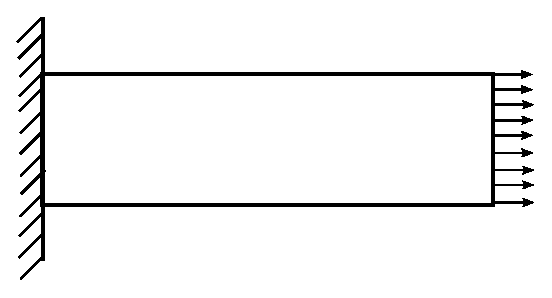
\includegraphics[width=8cm]{Figs/tension-simple}
  \put(-140,60){$E,\nu$}
  \put(3,60){$\sigma_0$}
  \caption{An isotropic material under simple
    tension} \label{fig-simple-tension}
\end{figure}
%
The expected tension at the end of the rod is
%
\begin{align}
  \delta l = \frac{ L \sigma_0 }{E} =\frac{20 \times 1000}{10^6} = 0.02   
\end{align}
%
The numerical value I got for the tension at the central point of the
material on the right hand side is $0.02$.
%
\begin{figure}[h]
  \centering
  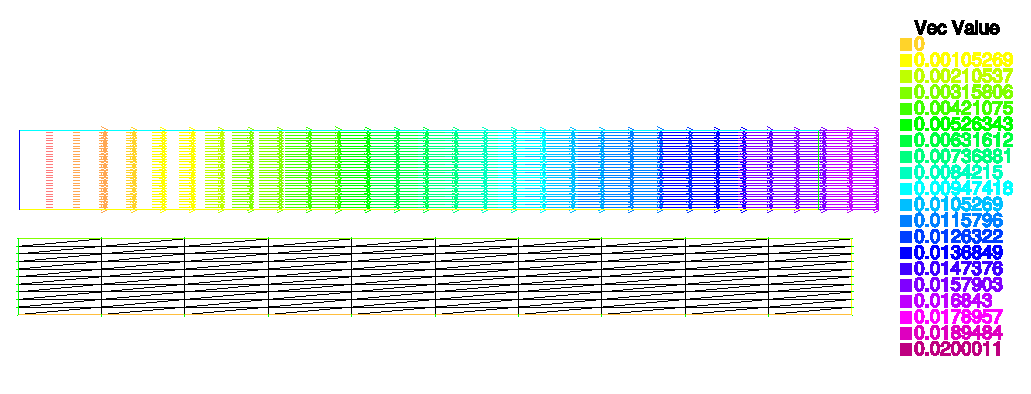
\includegraphics[width=17cm]{Figs/tension-result}
  \caption{Simulation result of a rod under tension} \label{fig-tension-result}
\end{figure}

\section{Random Network}
%
Consider the following network of pipes
%
\begin{figure}[h]
  \centering
  \includegraphics[width=12cm]{./grid.eps}
  \caption{A random grid of pipes} \label{fig-grid}
\end{figure}
%
The diameter of each pipe is randomly chosen from a Gaussian
distribution. The Darcy law in each pipe reads as
%
\begin{align}
  \frac{\Delta P}{L}  = \frac{128}{\pi} \frac{\mu Q}{d^4} 
\end{align}
%
where $\Delta P$ is the pressure difference on both sides of the pipe,
$L$ is the length of the pipe, $\mu$ is viscosity, and $d$ is the
diameter of the pipe. 













%\setcounter{page}{1}

\small{
\bibliography{./library.bib}}

\end{document}
